% ---------------------------------------------------------------
% Incluyo clase personalizada
\documentclass[a4paper]{styles/clase_fiuba}

% ---------------------------------------------------------------
% Configuracion caratula
\newcommand{\codigoMateria}{66.09 / 86.07}
\newcommand{\nombreMateria}{Laboratorio de Microprocesadores}

\newcommand{\descripcionTP}{Controlador de un actuador electrodinámico aplicado a interferometría dinámica}
\newcommand{\tituloTP}{Informe de Anteproyecto}

\newcommand{\facultad}{Facultad de Ingeniería}
\newcommand{\universidad}{Universidad de Buenos Aires}
\newcommand{\cuatrimestre}{1er Cuatrimestre de 2016}

\usepackage{styles/estilo_fiuba}

% ---------------------------------------------------------------
% Archivos bibliografia
\addbibresource{bibliografia.bib}

% ---------------------------------------------------------------
% Inicio documento
\begin{document}
% ---------------------------------------------------------------
% Caratula e índice
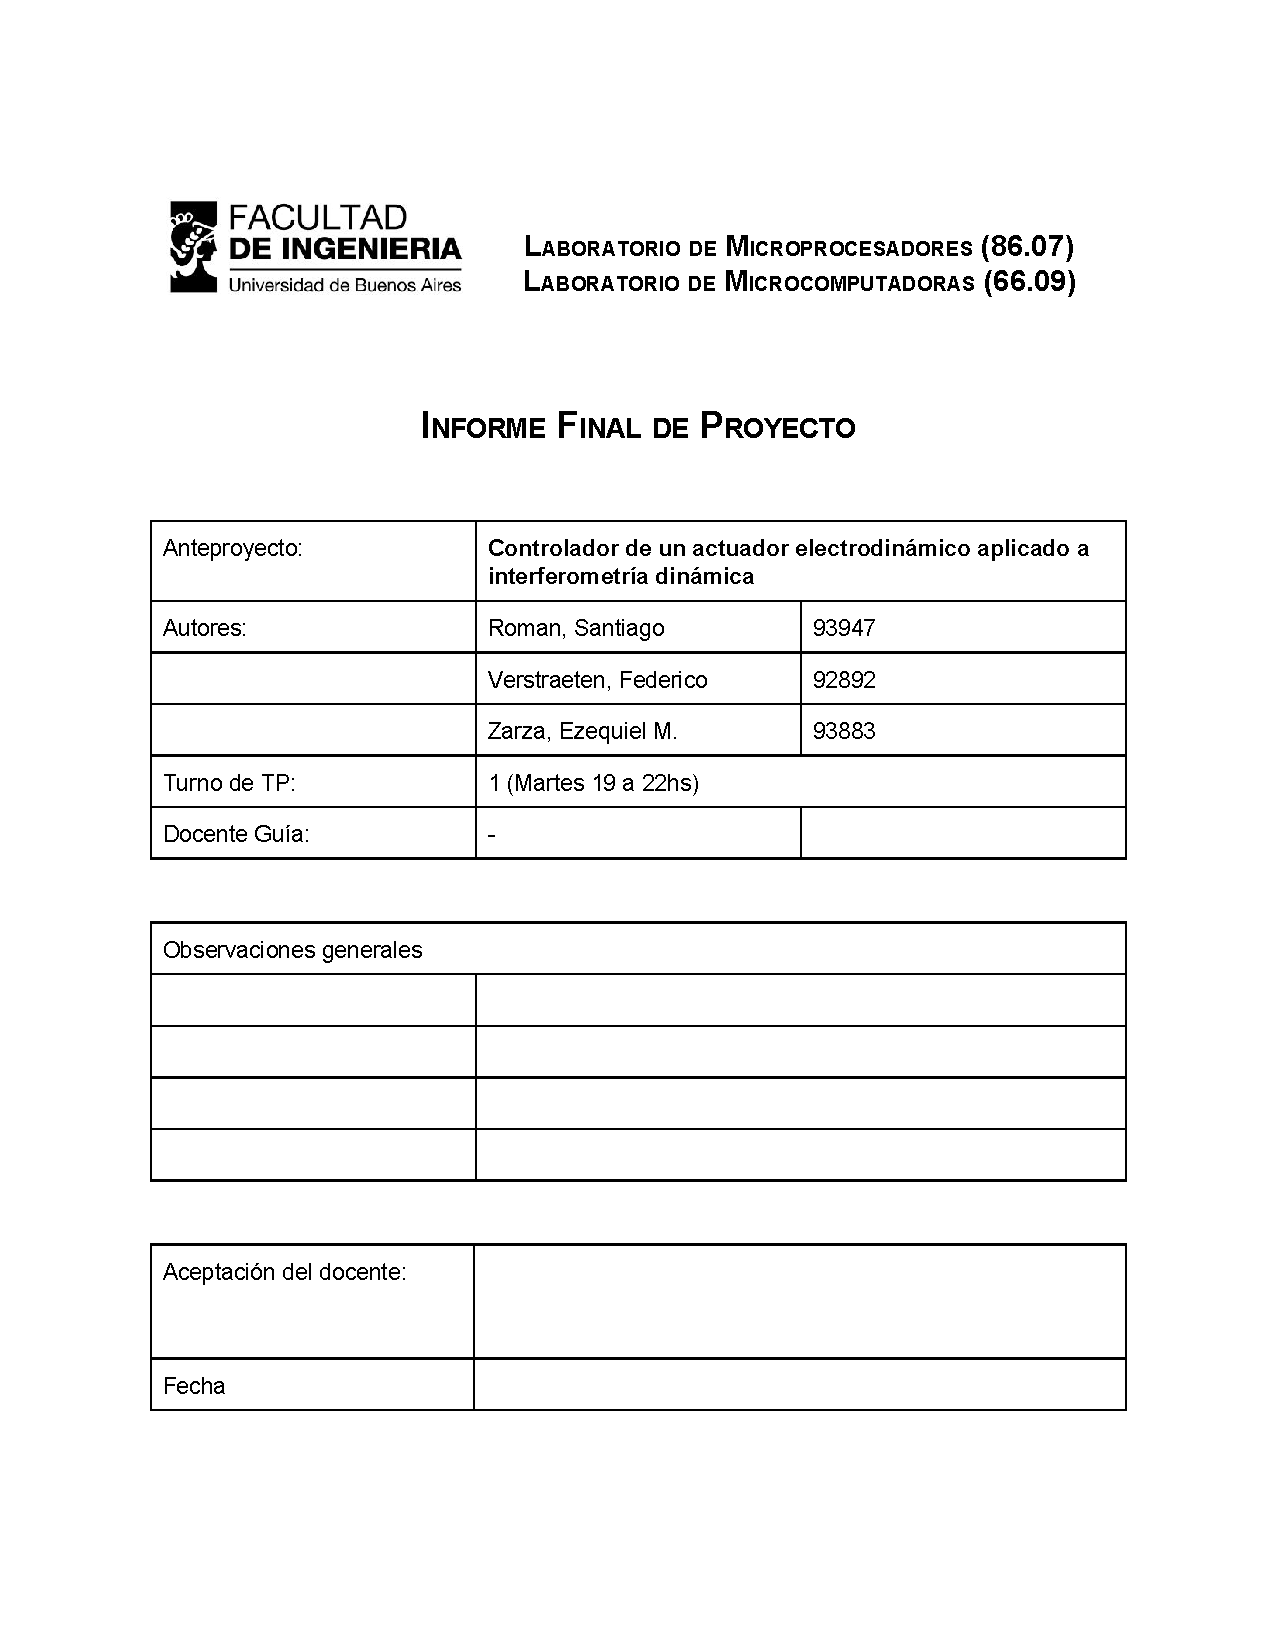
\includepdf[pages={1}]{Caratula_Informe_Final.pdf}
\clearpage

\pagenumbering{Roman}

\tableofcontents
\clearpage
% ---------------------------------------------------------------
% Cuerpo del informe.
\pagenumbering{arabic}
\pagestyle{fancy}

\section{Objetivos}
\label{sec:objetivos}
Un actuador es un dispositivo capaz de transformar energía (eléctrica para nuestro caso de interés) en la activación de un proceso con la finalidad de generar un efecto sobre un proceso automatizado. Un controlador se encarga de enviar ordenes al actuador con las cuales se activa un elemento final de control. Un ejemplo de actuador utilizado frecuentemente son los actuadores piezoeléctricos, los cuales producen una deformación mecánica sobre el material piezoeléctrico a partir de la aplicación de un campo eléctrico externo y viceversa. Estos tipos de actuadores pueden funcionar como por ejemplo, microposicionadores.
Para este proyecto se busca diseñar un actuador que se utilizará en un esquema interferométrico, más precisamente en un interferómetro de Michelson. Este tipo de esquema se describe en la figura \ref{fig:interferometro}.

\begin{figure}[H]
  \centering
  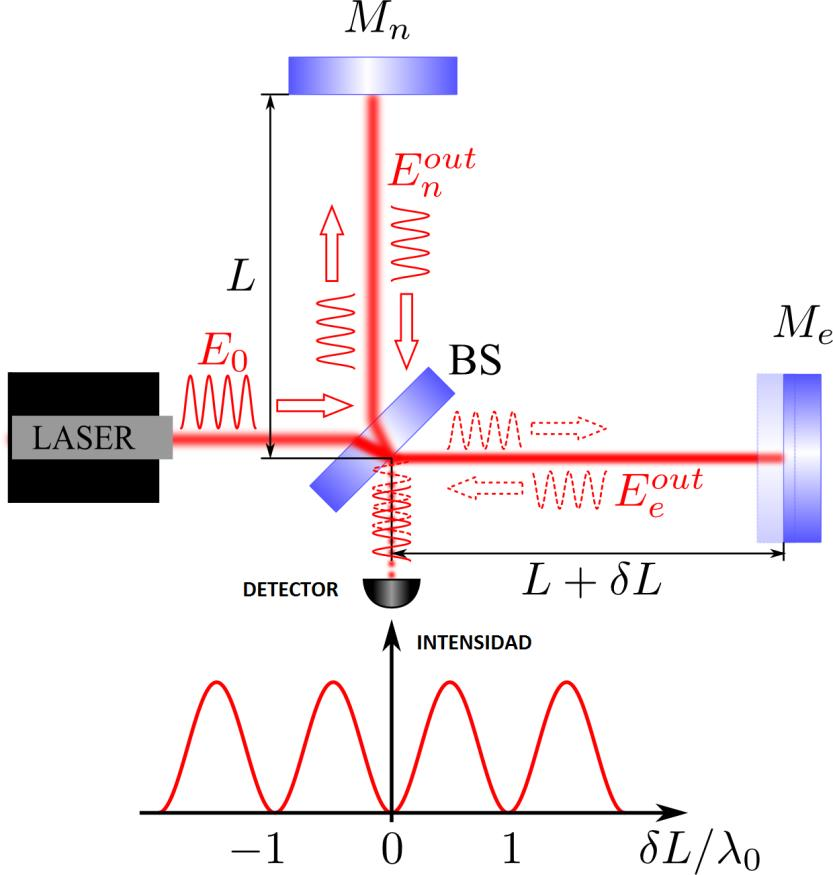
\includegraphics[width=0.6\textwidth]{images/interferometro_michelson.png}
  \caption{Interferómetro de Michelson}
  \label{fig:interferometro}
\end{figure}

Mediante un divisor de haz ($BS$), se superponen dos campos proveniente de un fuente monocromática y coherente($laser$). El campo que se desvía hacia la rama superior se refleja mediante un espejo fijo ($M_n$) mientras que el campo que se desvía hacia la derecha se refleja en un espejo móvil ($M_e$). De esta manera, los campos reflejados se dirigen hacia la rama inferior, donde se superponen en un fotodetector por medio del cual se puede registrar la intensidad de estos dos campos superpuestos. El modelo de esta intensidad es el siguiente:

\begin{equation}
I(t) = A + B \enspace cos[\frac{4 \pi}{\lambda_0} (L_1 - (L_2 + \delta L(t)))]
\end{equation}

De esta manera, con la ayuda del fotodetector se puede medir la intensidad producida por la diferencia de camino óptico ($\delta L$). si las ramas del interferómetro tienen la misma distancia (es decir, $L_1 = L_2 = L$), la intensidad registrada sólo depende del movimiento del espejo móvil $\delta L$.

Por lo tanto: Existe una variación de la intensidad detectada producto del desplazamiento del espejo móvil. Si conocemos $A$, $B$ y la longitud de onda de la fuente es posible recuperar la información del desplazamiento producido por $M_e$ midiendo la intensidad en el detector. Claramente este proceso también puede aplicarse de manera inversa, esto es si podemos controlar con una resolución elevada la posición del espejo podemos determinar la longitud de onda de la fuente lumínica y los parámetros $A$ y $B$.

\section{Descripción}
\label{sec:descrip}
En este caso particular, dado que se utiliza un esquema interferométrico como el de Michelson, puede no ser necesario contar con transductores tan precisos como los piezoeléctricos, pudiéndose optar por alternativas que resulten más económicas.
De esta manera, en el presente trabajo nos planteamos obtener un método de transducción eléctrica-mecánica a partir de dispositivos de uso común cuyo sistema de control incluya la posibilidad de definir el tipo de desplazamiento que se desea utilizar por medio de Matlab. Particularmente, se buscará generar el desplazamiento de un espejo conectándolo a un parlante o altavoz, el cual será controlado por Matlab mediante la presencia de un microcontrolador como intermediario entre estos.

Se comenzará por analizar el sistema interferométrico utilizado para poder definir los parámetros más significativos de control que se requieren (desplazamiento necesario, aspectos mecánicos y de diseño, opciones de control, etc.). Finalmente, una vez diseñados e implementados, se caracterizarán mecánicamente con la misma instrumentación interferométrica para obtener una evaluación de la performance del sistema completo.

\section{Especificaciones}
\label{sec:especif}
En cuanto a lo que se refiere al hardware propio del proyecto, es decir el parlante que se encarga de transformar energía eléctrica y producir un desplazamiento físico; tras realizar diferentes pruebas con varios modelos de parlantes elegimos aquel que mostró una mayor respuesta lineal en conjunto con un desplazamiento en una sola dirección . Esto último es de especial importancia ya que existe la posibilidad de que algunos parlantes generen un desplazamiento oblicuo.

El elemento central de control del actuador electrodinámico es el microcontrolador ATMega32. La elección de este tuvo como premisa fundamental de que disponga de la suficiente memoria volátil (RAM) y la necesaria para alojar el programa que ejecutará finalmente (ROM).\\
Estas consideraciones se deben a que en este trabajo utilizamos memoria ROM para almacenar las Lookup Tables de la función seno pre cargada (es decir, se encuentran guardadas una determinada cantidad de muestras de cada función que en total forman un período de las mismas). Por otro lado, la memoria RAM se utiliza principalmente para almacenar las muestras correspondientes a la señal generada en Matlab, la cual se exporta al microcontrolador por medio del protocolo de comunicación serie USART. \\
Desde ya, dado que solamente vamos a utilizar señales periódicas, es posible generar una señal continua a lo largo de un período de tiempo contando únicamente con las muestras correspondientes a un período.

Otro punto importante de la elección del microcontrolador en cuestión es que debe contar con la cantidad suficiente pines I/O para poder relacionarse con los distintos periféricos externos que conforman a este proyecto. A continuación mostramos una tabla con la cantidad de pines que requiere cada parte del proyecto:

\begin{table}[H]
  \centering
  \begin{tabular}{ll}
    \toprule
    Elemento & \# pines \\
    \midrule
    Parlante (DAC) & 8 \\
    Display & 7 \\
    Pulsadores & 4 \\
	Matlab/USART ($T_X$ y $R_X$)  & 2 \\
	Módulo de detección (ADC) & 1 \\
    Cristal & 2 \\
    \midrule
    Total & 24 \\
    \bottomrule
  \end{tabular}
  \caption{Análisis de la cantidad de pines I/O requeridos para cada parte del programa.}
  \label{table:pines}
\end{table}

La versión final del proyecto se presenta ensamblada sobre una placa experimental.\\
La fuente de alimentación es provista por una placa conversora USB/Serie, la cual cuenta con salidas de \SI{5}{\volt} y \SI{3.3}{\volt}. Esto permite evitar el uso de una fuente separada para poder alimentar al microcontrolador.\\

Al iniciar el programa se muestra el menú principal en el display LCD, por el cual puede desplazarse utilizando los botones \textit{Arriba} y \textit{Abajo}. Para  seleccionar alguna de las opciones se utiliza el botón \textit{Enter} y para regresar al menú principal el restante, el cual ejecuta una interrupción externa y regresa al menú principal.\\
\\

Por último, se utiliza un módulo de detección de intensidad, el cual permite medir este parámetro y mostrar un promedio del mismo en el display. El haz de luz al cual se calcula la intensidad sale de colocar un divisor de haz extra en la última rama del interferómetro (ver imágen \ref{fig:interferometro}), a partir de la cual queda colocado en una sección el detector que va conectado al osciloscopio que ya se mencionó anteriormente, y en la otra el módulo de detección que esta conectado al microcontrolador.

\section{Periféricos Principales}
\label{sec:perif}

\begin{itemize}
\item Placa conversora USB a Serie: es necesaria para poder conectar a una computadora via puerto USB y que la computadora sea capaz de reconocer al dispositivo como un puerto serie virtual. De esta manera es posible utilizar las funciones de Matlab que permiten enviar datos a través de un puerto serie. Además estas placas incluyen conexiones para alimentar al microcontrolador con lo cual se lo podría energizar solamente con la conexión a una computadora sin necesidad de utilizar un cable adicional. En el mercado argentino se encuentran este tipo de placas basadas en dos integrados distintos: Cp2102 y CH340, cuyas correspondientes hojas de datos se incluyen a continuación:
\begin{itemize}
\item \href{https://www.olimex.com/Products/Breadboarding/BB-CH340T/resources/CH340DS1.PDF}{\color{blue} Hoja de datos CH340}
\item \href{https://www.sparkfun.com/datasheets/IC/cp2102.pdf}{\color{blue} Hoja de datos Cp2102}
\end{itemize}

\begin{figure}[H]
  \centering
  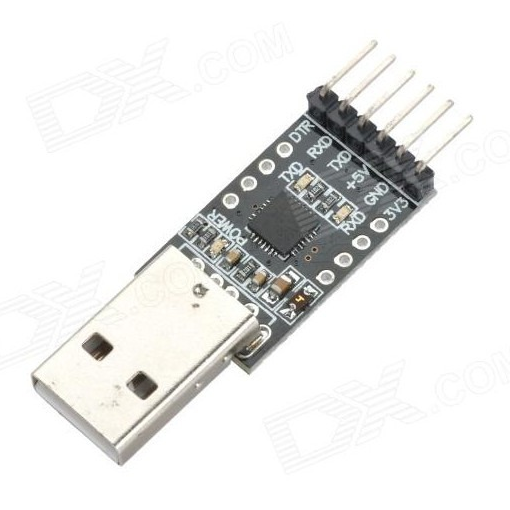
\includegraphics[width=0.6\textwidth]{images/conversor_usbttl.png}
  \caption{Ejemplo de placa conversora usb a serie}
  \label{fig:usbattl}
\end{figure}

\item Parlante o Altavoz: Necesario para poder generar el desplazamiento en el espejo. Será necesario evaluar distintos tipos de parlantes para entender cuál resulta útil para cumplir nuestros objetivos.
\item Diseñar un soporte para el dispositivo en su totalidad de manera tal que pueda ser utilizado en una mesa antivibratoria en la cual se encuentra instalado el interferómetro. En este soporte estará colocado el parlante con un espejo pegado al mismo.
\end{itemize}

\section{Diagrama de bloques preliminar}
\label{sec:diag_bloq}
Quisque erat metus, cursus in pellentesque a, lobortis in diam. In hac habitasse platea dictumst. Nunc ac mauris ac felis luctus varius vel ac dui. Sed feugiat ullamcorper dolor, at aliquet ex ultricies id. Vivamus sed nulla sit amet magna consectetur elementum. Nulla sed lorem quis neque euismod feugiat et id leo. Aliquam placerat dapibus turpis. Cras sollicitudin vitae ante a feugiat. Fusce interdum quam a enim ultrices tristique. Vivamus sed volutpat turpis. Fusce feugiat velit id magna finibus convallis. Nulla malesuada leo id fermentum condimentum. Sed ultricies ornare metus varius varius. 

\section{Diagrama de flujo (firmware)}
\label{sec:diag_flujo}
A continuación se presenta el Diagrama de flujo correspondiente al Menú principal del proyecto. A través de este, que funciona como interfaz con el Usuario, se puede seleccionar los distintos modos de operación que puede ejecutar el microcontrolador.

\begin{itemize}
\item Seno: generación de una señal senoidal precargada en memoria del programa (ROM), con una Frecuencia y Amplitud prefijadas.
\item Dientes de Sierra: generación de una señal Dientes de Sierra, a partir de una función implementada en Assembly, con una Frecuencia y Valor Pico prefijados.
\item Matlab: el programa abre un canal de comunicación de transmisión Serie entre Matlab y el Microcontrolador, donde este último recibe datos, los almacena en RAM, procesa y genera la salida con los datos acondicionados entre 0 y 255 valores.
\item Intensidad: Este modo de operación permite al Microcontrolador medir la intensidad lumínica de las ramas del Interferómetro. Esto se hace mediante un fotodiodo en serie con una resistencia, la cual esta conectada al conversor Analogico-Digital interno del Microcontrolador. 
\end{itemize}

Las señales se generaran de forma continuada hasta que el usuario detiene el proceso mediante una Interrupción Externa activada al presionar un pulsador, la cual salta el programa al Inicio del Menú.
Dichas señales se generan en un Puerto establecido como salida, el cual tiene conectado un conversor Digital-Analógico (DAC).

\begin{figure}[H]
  \centering
  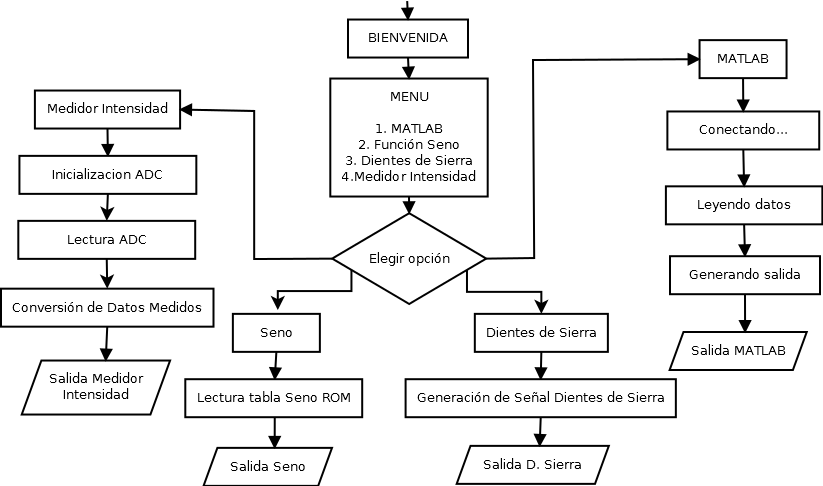
\includegraphics[width=1.0\textwidth]{images/flujo_menu_informe_v1.png}
  \caption{Diagrama de flujo del menú principal.}
  \label{fig:Diagrama de flujo}
\end{figure}

\section{Esquemático}
\label{sec:esquematico}
A continuación se muestra el esquemático realizado en Proteus.

\begin{figure}[H]
  \centering
  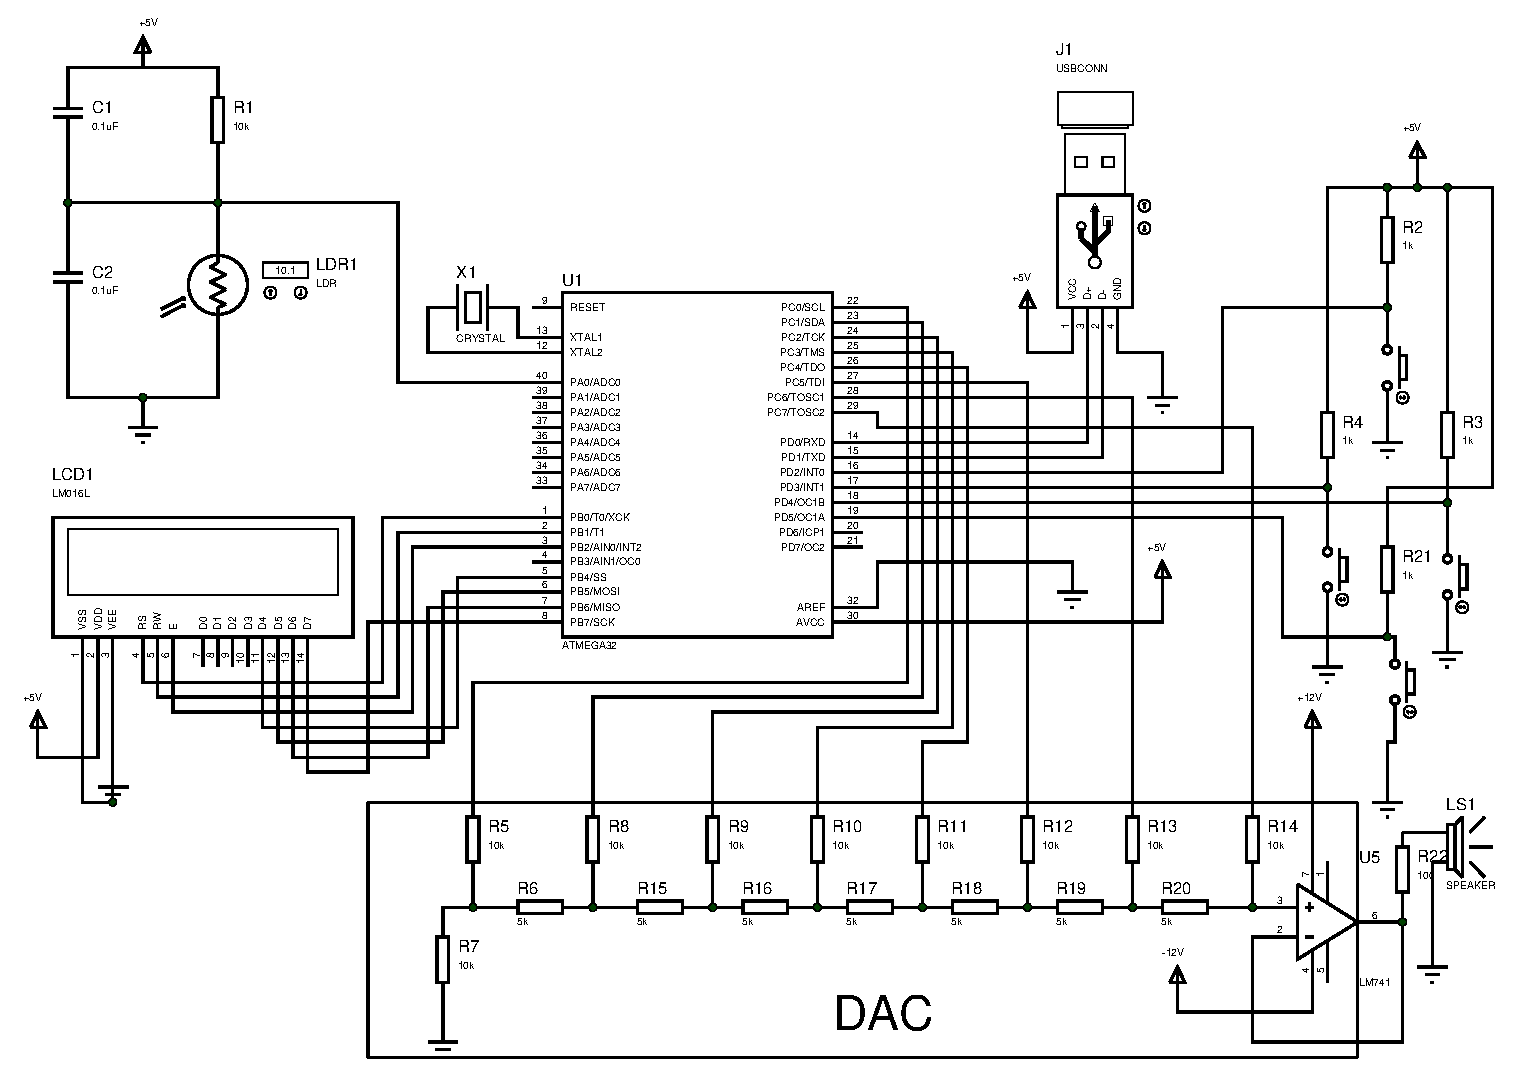
\includegraphics[width=1.0\textwidth]{images/ProyectoLaboratorioMicroprocesadores.PDF}
  \caption{Esquemático del proyecto en Proteus.}
  \label{fig:Esquemático}
\end{figure}

\section{Listado de componentes y costos estimados}
\label{sec:componentes}

\begin{table}[H]
  \centering
  \begin{tabular}{ll}
    \toprule
    Componente & Costo estimado \\
    \midrule
    Microprocesador ATMega328p & \$ 110 \\
    Placa experimental & \$ ?? \\
    Soporte & \$ ?? \\
    Placa USB a Serie & $\approx$ \$ 120 \\
	Parlante & \$ ?? \\
    \midrule
    Total & \$ ?? \\
    \bottomrule
  \end{tabular}
  \caption{Costos estimados para la realización del proyecto.}
  \label{table:costos}
\end{table}

\section{Resultados}
\label{sec:resultados}

Tras haber verificado el correcto funcionamiento de cada parte que conforma el proyecto se realizó una implementación del mismo en una placa experimental. En la figura \ref{fig:placa} se puede ver el resultado final de la misma.

\begin{figure}[H]
  \centering
  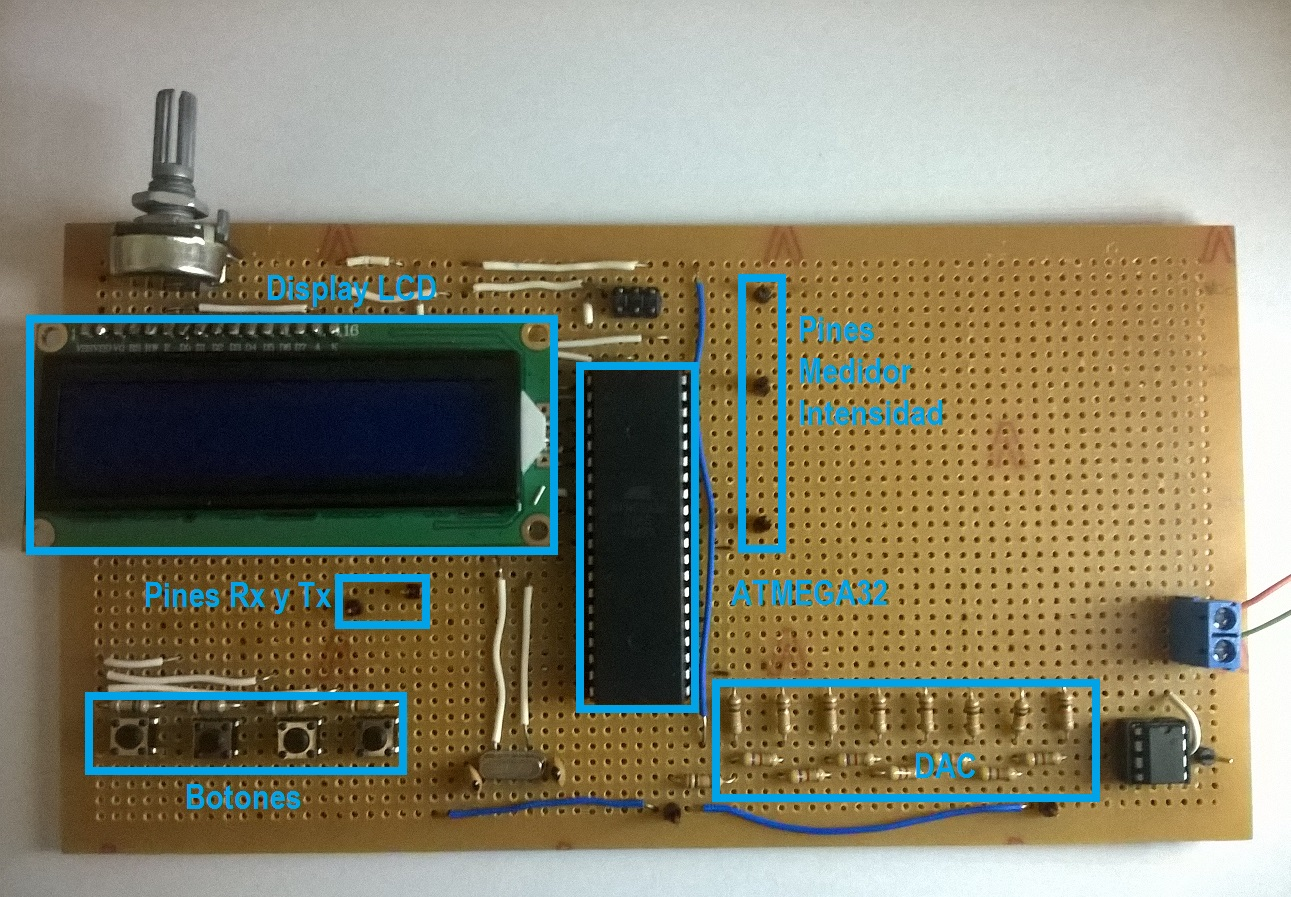
\includegraphics[width=1.0\textwidth]{images/placa.jpg}
  \caption{Versión final del proyecto implementado en una placa experimental.}
  \label{fig:placa}
\end{figure}

Se realizaron mediciones en el osciloscopio de las salidas que se obtienen para las funciones seno y una rampa y en las figuras \ref{fig:salida_rampa} y \ref{fig:salida_seno} se muestran capturas de pantalla del osciloscopio para cada señal.

\begin{figure}[H]
  \centering
  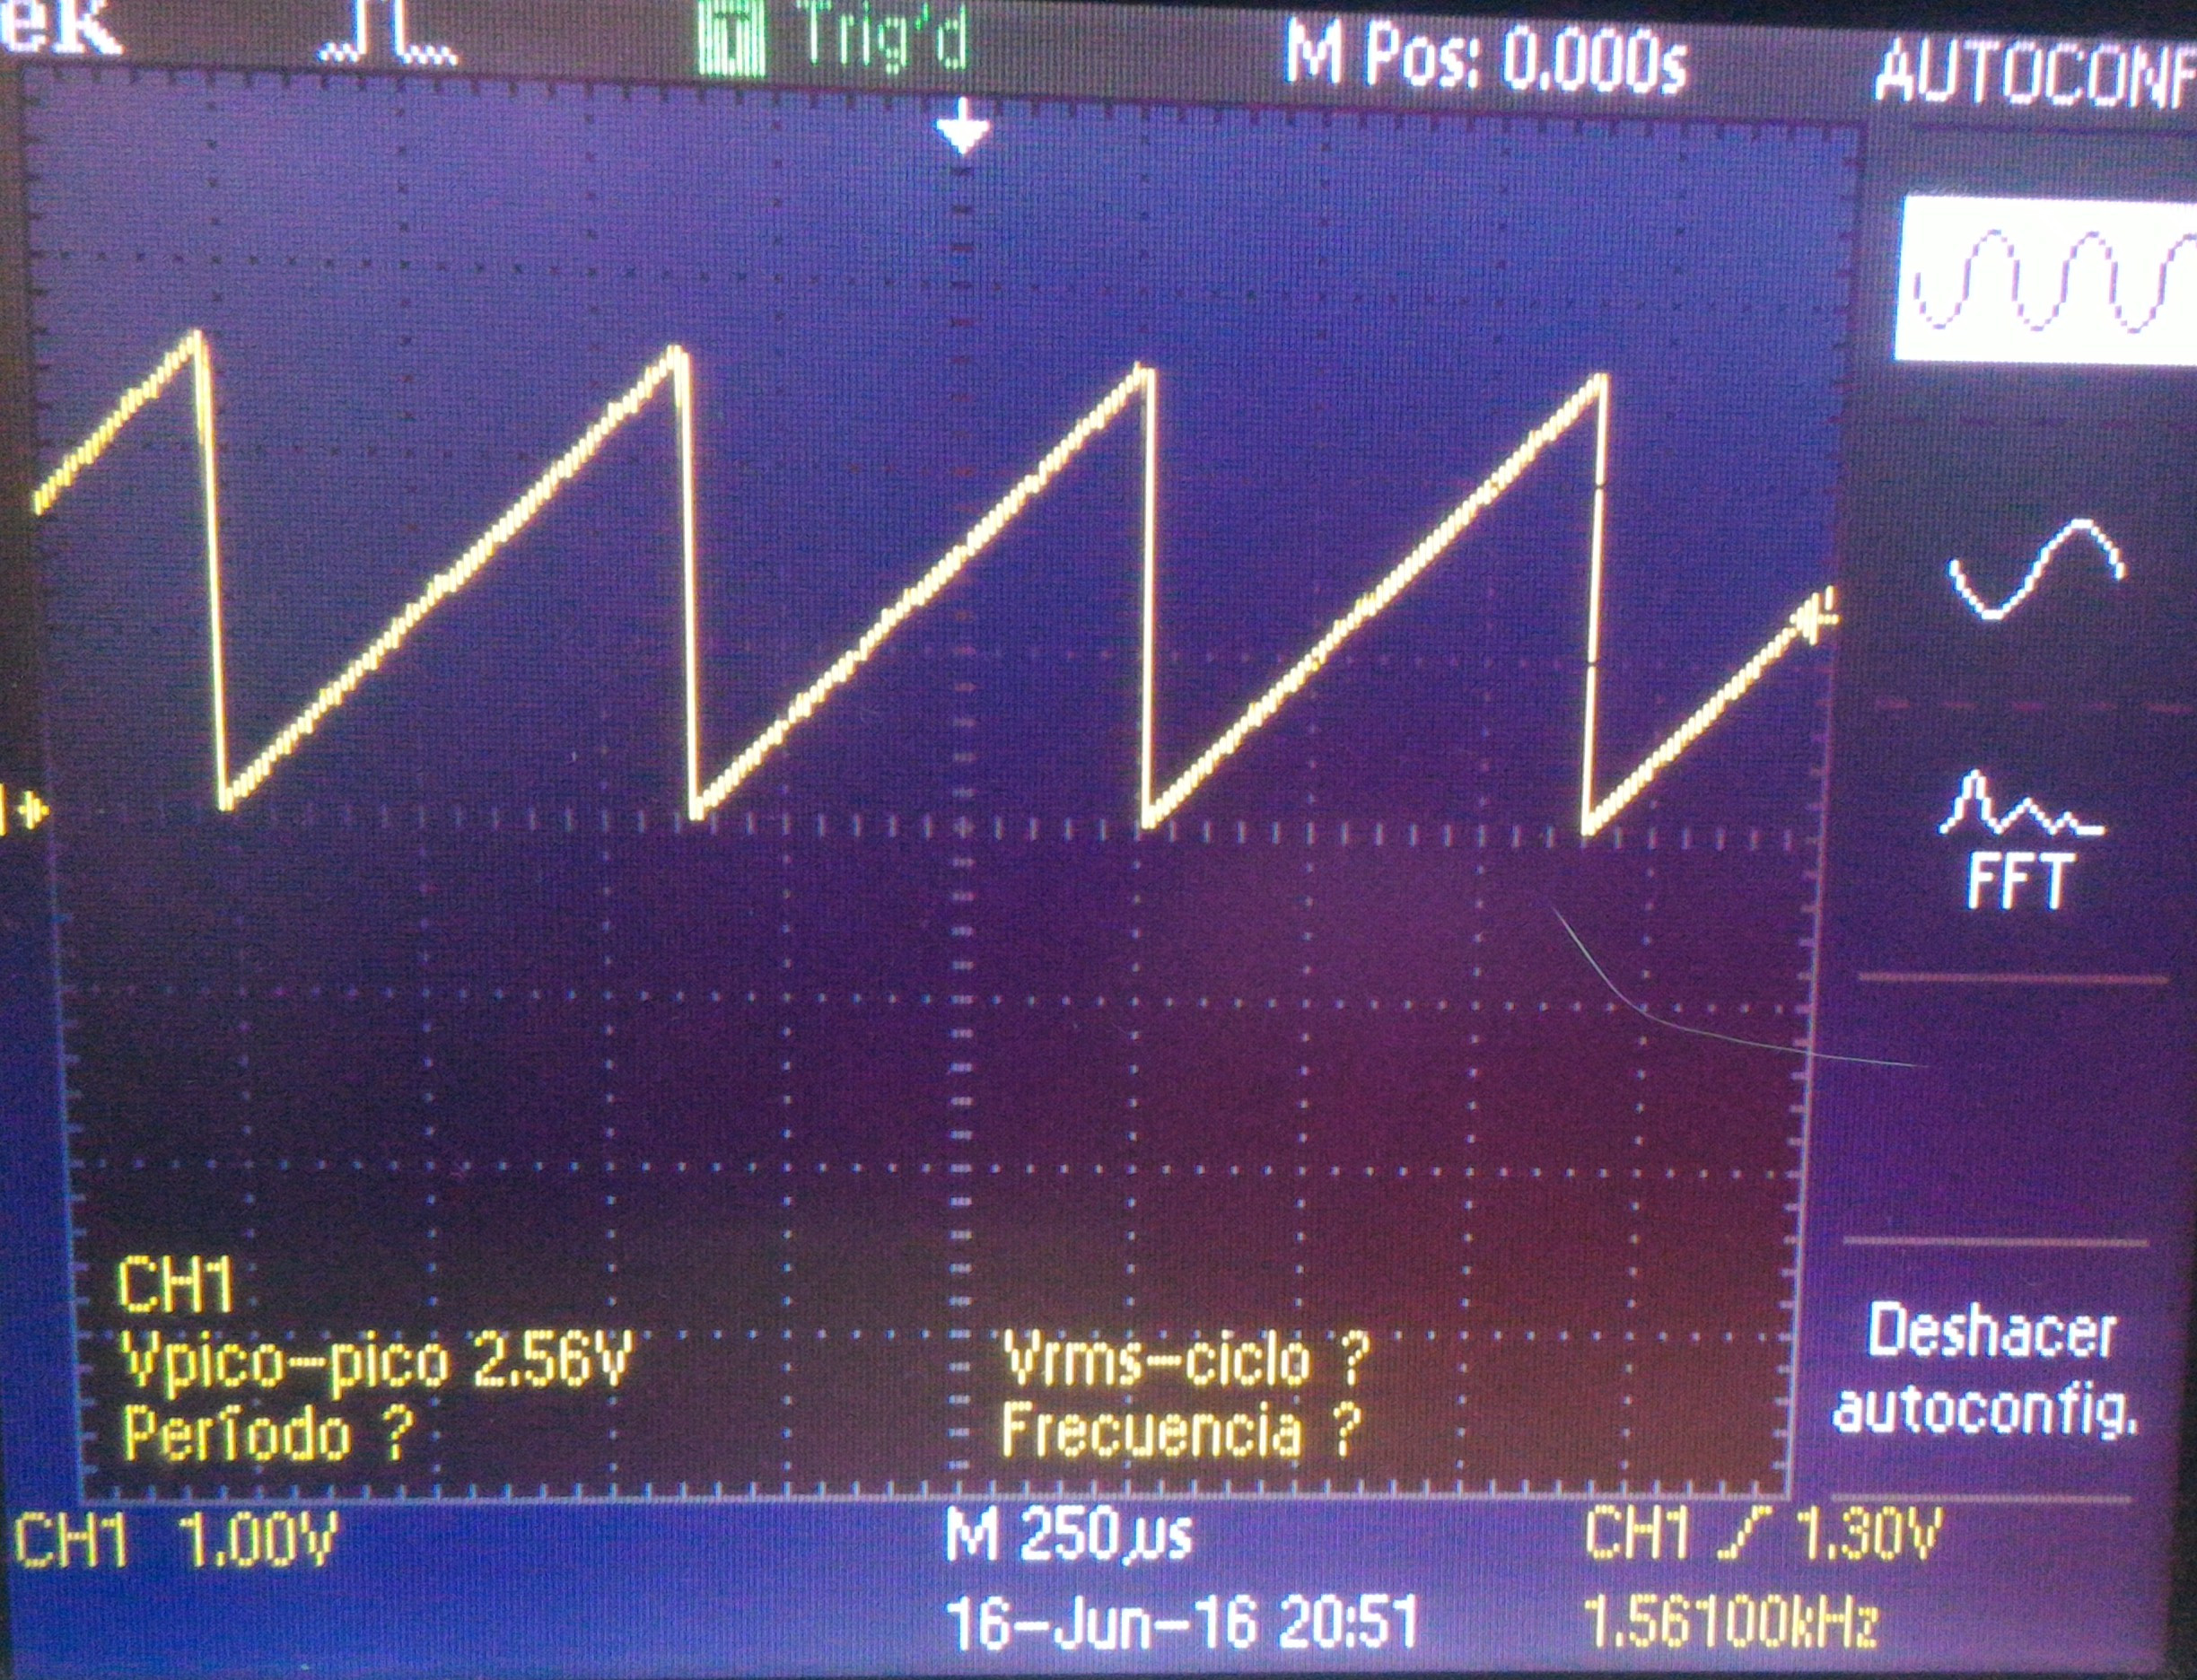
\includegraphics[width=0.8\textwidth]{images/resultados_rampa_precargadav2.jpg}
  \caption{Salida obtenida para la función dientes de sierra/rampa.}
  \label{fig:salida_rampa}
\end{figure}

\begin{figure}[H]
  \centering
  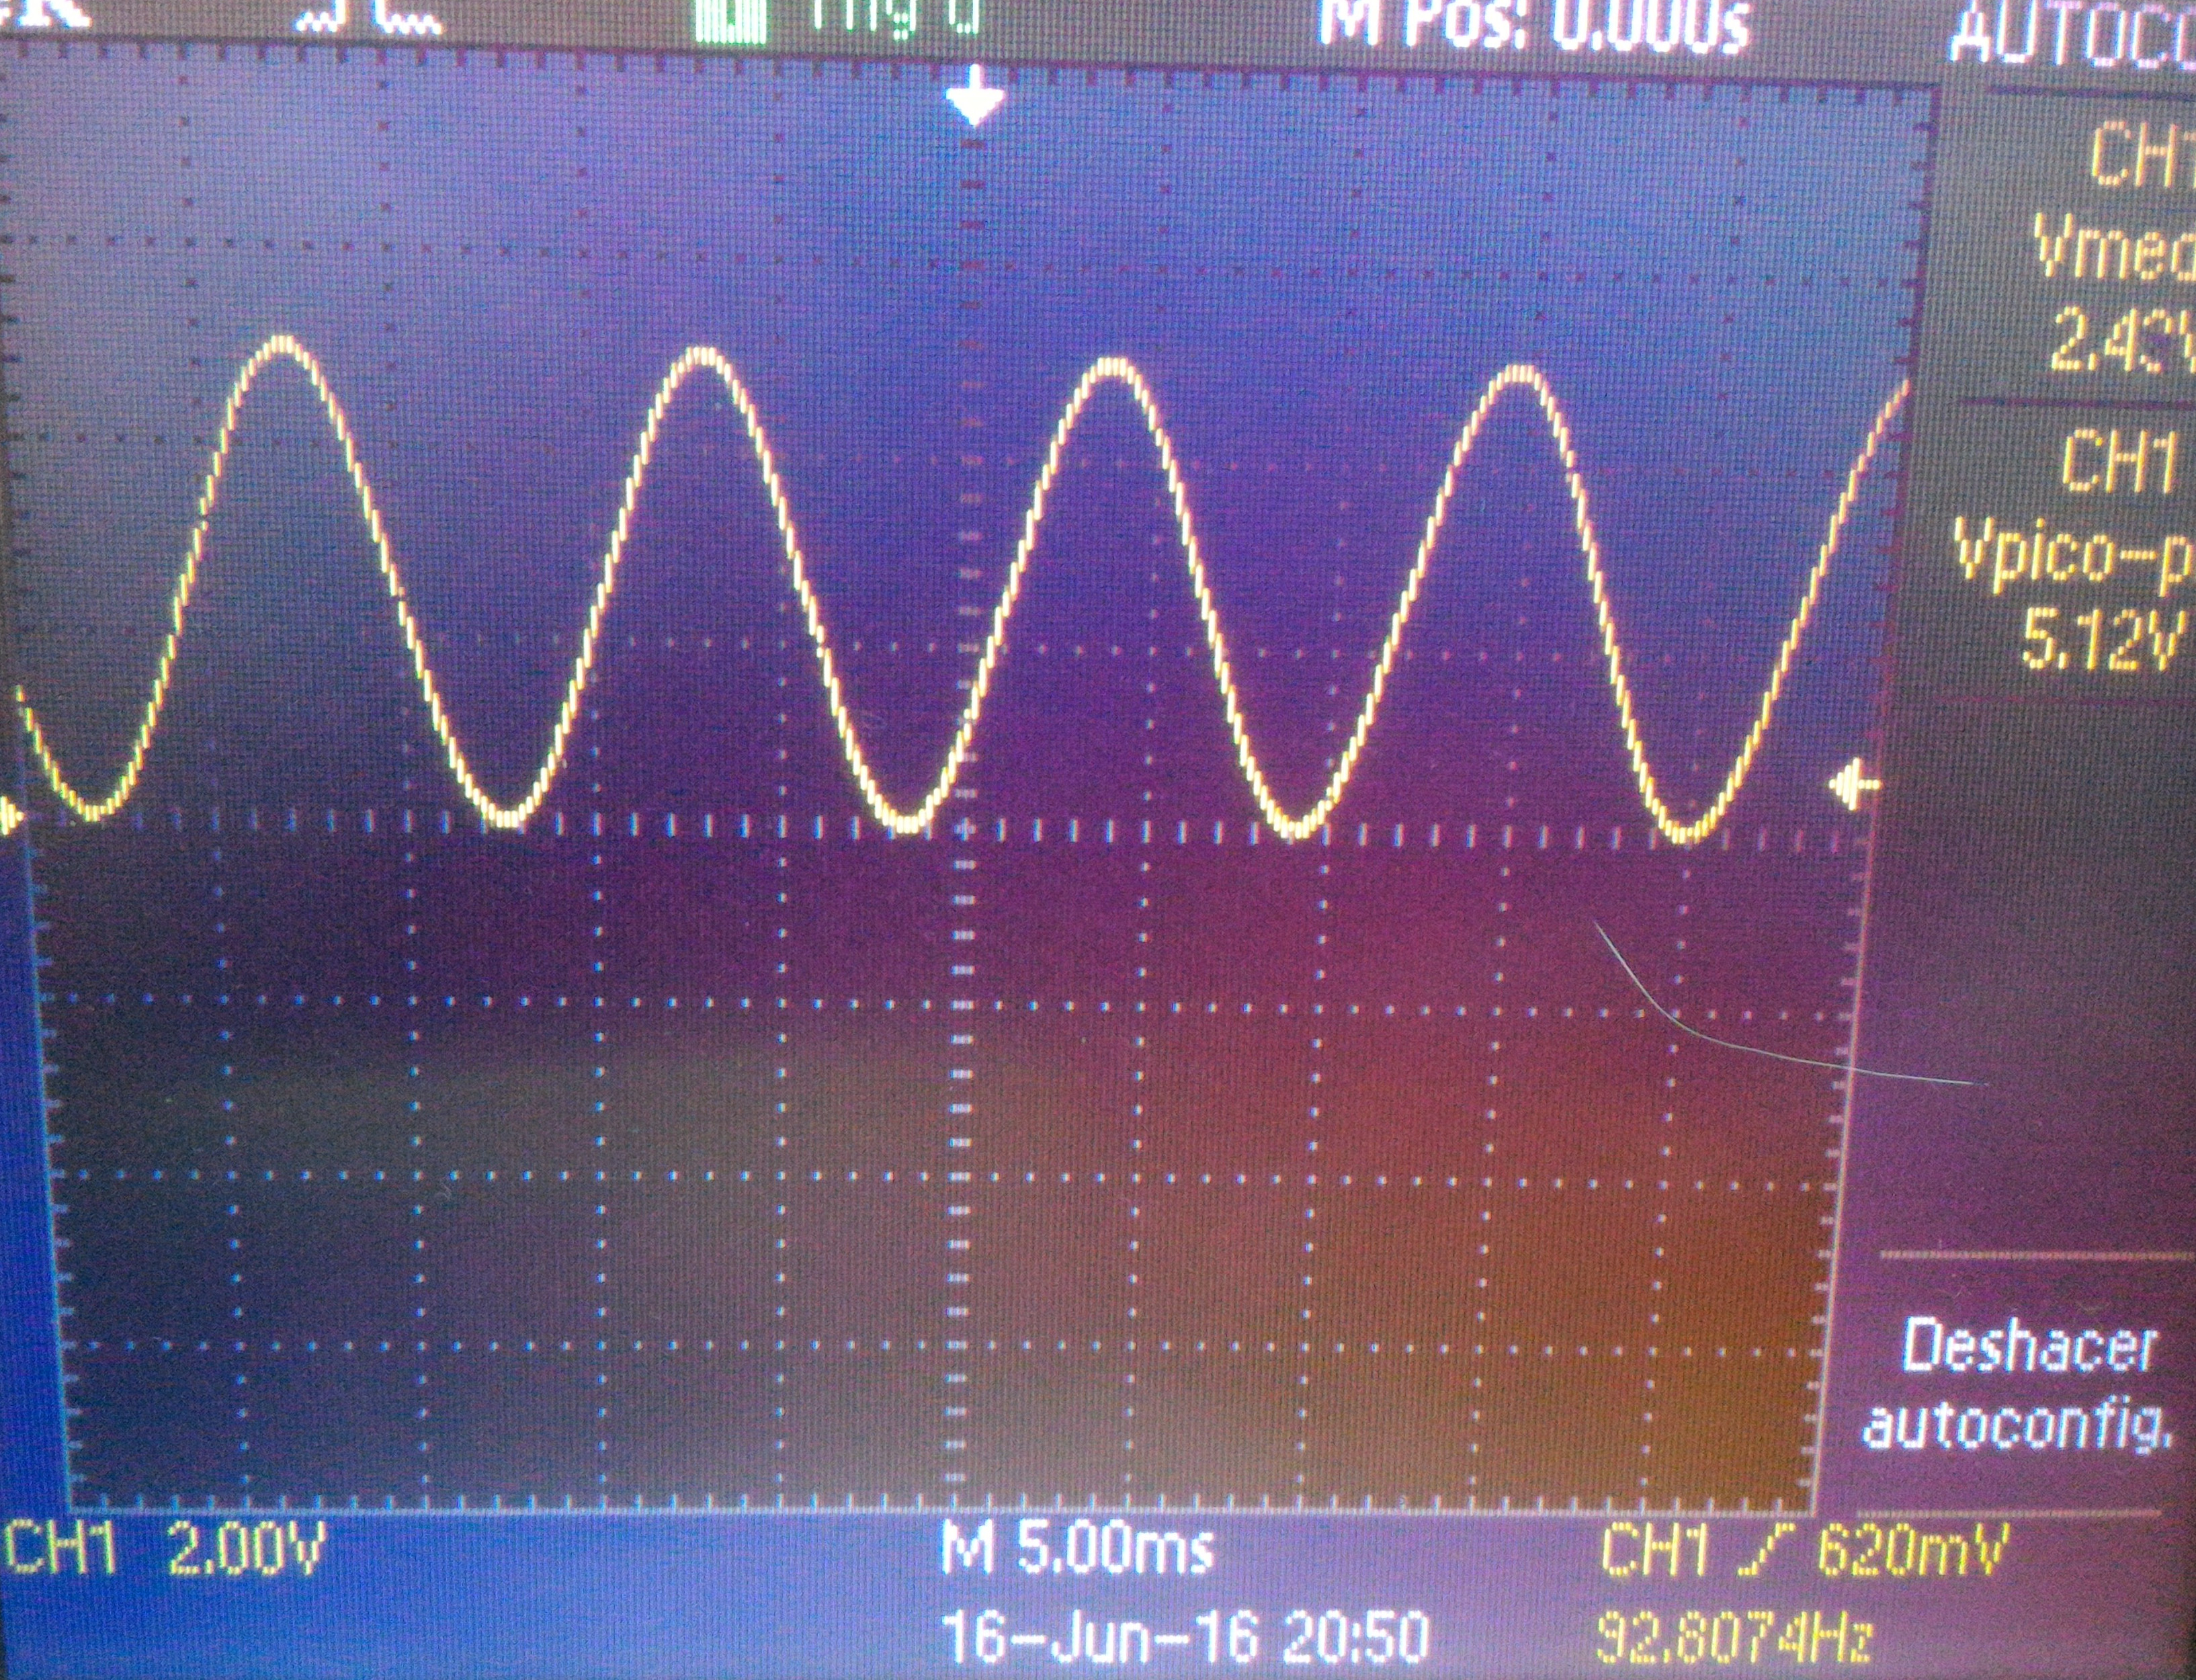
\includegraphics[width=0.8\textwidth]{images/resultados_seno_precargadav2.jpg}
  \caption{Salida obtenida para la función seno.}
  \label{fig:salida_seno}
\end{figure}

En cuanto a los riesgos que se podían presentar que analizamos en el informe de anteproyecto es posible aclarar que el parlante utilizado para poder generar un desplazamiento físico a partir de una señal eléctrica no tuvo problemas de alinealidad y pudo ser incluido en el esquema interferométrico sin mayores problemas. De todas formas, es necesario calibrar la señal de salida para poder obtener resultados óptimos cuando se lo usa en el esquema interferométrico.\\

\begin{figure}[H]
  \centering
  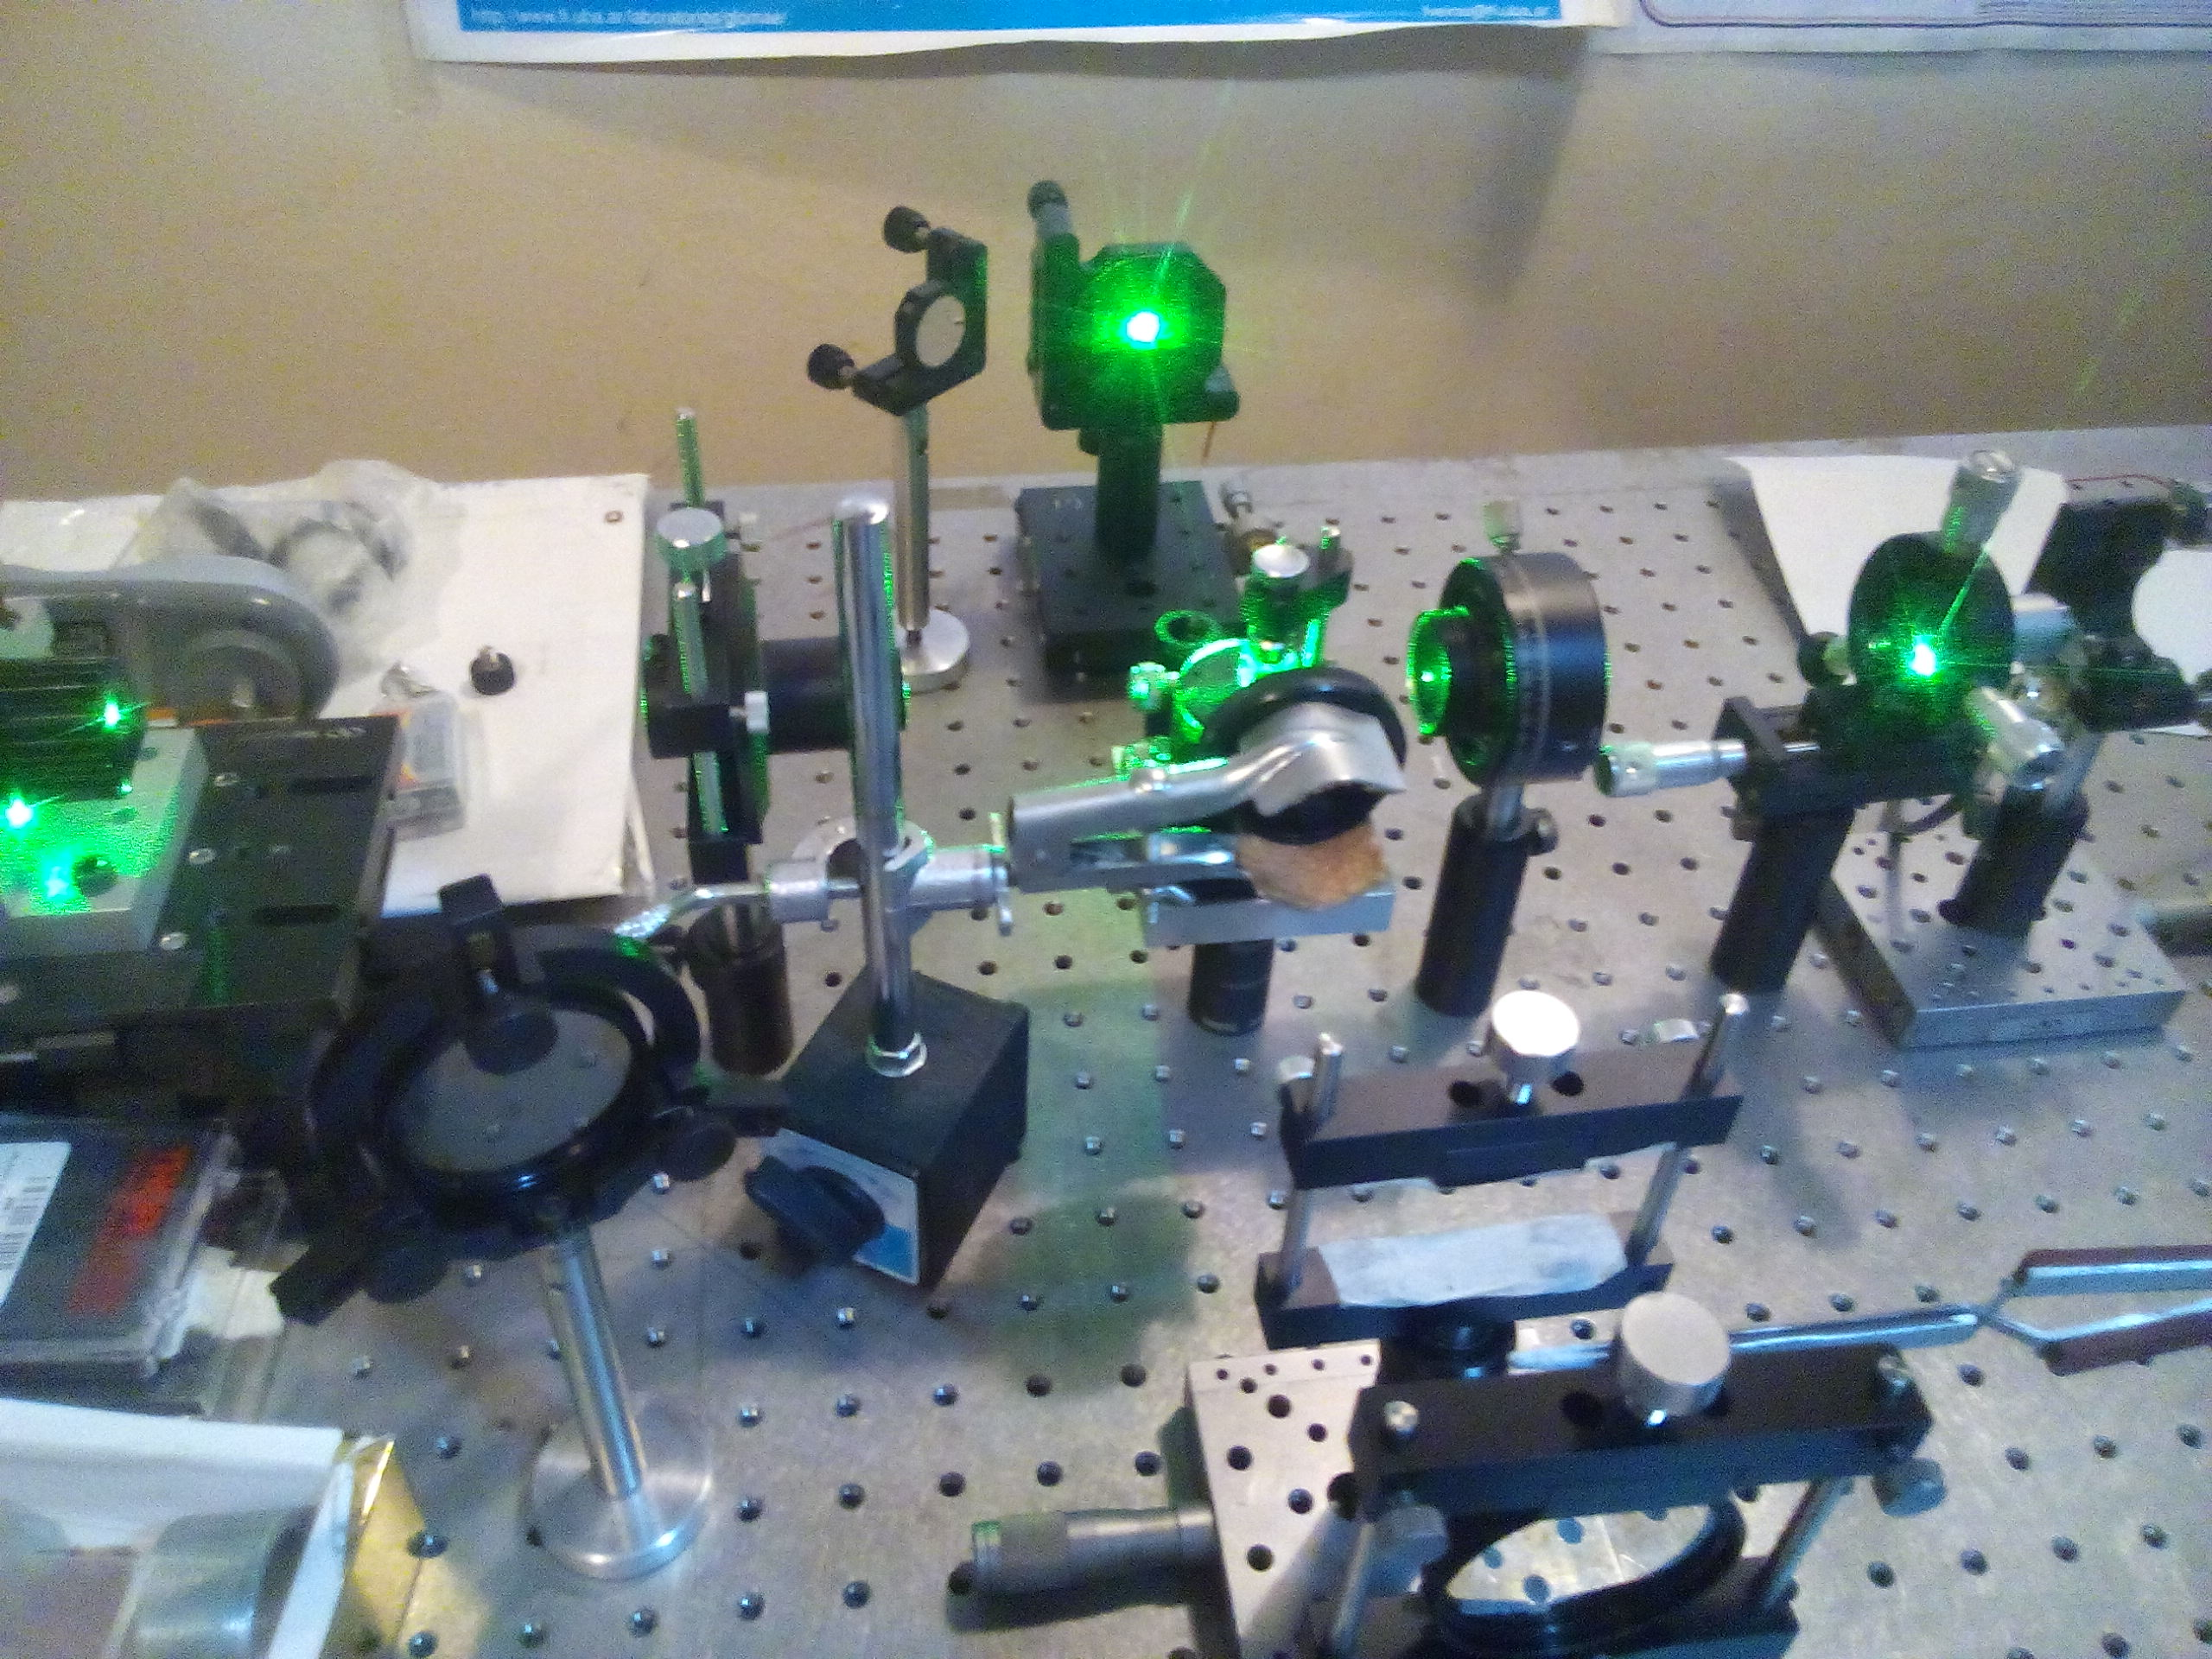
\includegraphics[width=0.8\textwidth]{images/interferometro2.jpg}
  \caption{Interferómetro encendido con el parlante en una de sus ramas}
  \label{fig:interferometro_encendido}
\end{figure}

Por otro lado, otro posible problema era el desarrollo del middleware para pasar las muestras de una señal de Matlab hacia el microcontrolador. Gracias a que Matlab cuenta de antemano con funciones diseñadas para poder comunicarse con un dispositivo serie fue muy sencillo crear un programa que tome muestras de una señal periódica y las envíe al microcontrolador.

Otra de las funciones del proyecto es la medición de intensidad lumínica, se realizaron diversas pruebas sencillas y se verificó el correcto funcionamiento ya que al dejar el módulo de detección completamente a oscuras el valor medido de potencia se vuelve nulo mientras que al utilizar un puntero laser el valor de potencia que se muestra en el display aumenta exponencialmente.

Finalmente, es importante aclarar que si bien es posible verificar el correcto funcionamiento de las diferentes funciones del dispositivo es necesario realizar diferentes experimentos a partir de las cuales va a ser necesario modificar el código del proyecto de manera tal que se logre una precisión mayor que permita que se pueda utilizar en una medición de laboratorio.

\section{Conclusiones}
\label{sec:conclusiones}

Primeramente se debe concluir que fue posible implementar correctamente en el proyecto todas las funciones que se plantearon en el informe de anteproyecto. Esto es, crear un menu para poder desplazarse a través de las diferentes opciones que modifican el modo de funcionamiento del dispositivo. Se puede seleccionar entre generar funciones seno o rampa precargadas en el microcontrolador, tomar una función enviada por medio del protocolo USART desde Matlab, y mostrar en el display la intensidad medida en el módulo de detección.

Entre una de las cosas más importantes que se aprendieron durante la realización de este proyecto es la correcta utilización de las hojas de datos que provee Atmel para sus microcontroladores AVR. Esto es de vital importancia ya que muchas veces existen errores que se pueden solucionar entendiendo cómo fue diseñado el microcontrolador. Un ejemplo de esto es que el microcontrolador ATMega32 cuenta activado por defecto la funcionalidad de debuggeo JTAG, la cual impide el correcto uso del puerto C y en caso de ser necesario hay que desactivar JTAG por medio del seteo de fusibles.

Este proyecto nos permitió aprender a utilizar diversas utilidades de los microcontroladores, entre las que se destacan el protocolo de comunicación serie USART, el conversor ADC, la configuración de interrupciones y el modo de comunicación con un display LCD externo.

% --------------------------------------------------
% Bibliografías
\printbibliography
%\clearpage
% --------------------------------------------------
% Fin del informee
\end{document}
